\chapter{Introduction} \label{chap:introduction}

Some \textbf{interesting} \textsf{introduction} and some \emph{interesting} reference.
\par\textbf{Bold} \textit{Italic} \textbf{\textit{BoldItalic}}
\par\textsf{Sans \textbf{Bold} \textit{Italic} \textbf{\textit{BoldItalic}}}
\par\texttt{Mono \textbf{Bold} \textit{Italic} \textbf{\textit{BoldItalic}}}

\begin{equation}
    \begin{pmatrix}
      1 & 2 & 3  \\
      1 & 2 & 3  \\
      1 & 2 & 3
    \end{pmatrix}
    = \left( \sum_{i=1}^{n-1} i \right)
    = \left( n \right)
\label{eq:first}
\end{equation}

\textcite{Walley2000} writes that \LaTeX\ is really good. \textcite{entrywithurl} agrees. Here's an abbreviation on \gls{ai}. If you want to add additional abbreviations, you can do that in the main file. Here's another abbreviation for \gls{moo}.

To reference figures, tables or sections, use \verb|\cref{label}|, see \cref{tab:citations}, \cref{fig:first_figure}, or the above equation \cref{eq:first}.

\begin{table}
\caption{Various literature citations.}
\begin{tabular}{L{.6\linewidth}L{.3\linewidth}}%
\toprule%
\lstinline|\cite{Walley2000}| & \cite{Walley2000} \\[0.5em]%
\lstinline|\cite{Walley2000,knauth2003prevcompmeasuresshiftwrk,yang2010wikipediacontrib}| & \cite{Walley2000,knauth2003prevcompmeasuresshiftwrk,yang2010wikipediacontrib} \\
\midrule%
\lstinline|\parencite{Walley2000}| & \parencite{Walley2000} \\[0.5em]%
\lstinline|\parencite{Walley2000,knauth2003prevcompmeasuresshiftwrk,yang2010wikipediacontrib}| & \parencite{Walley2000,knauth2003prevcompmeasuresshiftwrk,yang2010wikipediacontrib} \\
\midrule%
\lstinline|\autocite{Walley2000}| & \autocite{Walley2000} \\[0.5em]%
\lstinline|\autocite{Walley2000,knauth2003prevcompmeasuresshiftwrk,yang2010wikipediacontrib}| & \autocite{Walley2000,knauth2003prevcompmeasuresshiftwrk,yang2010wikipediacontrib} \\
\midrule%
\lstinline|\textcite{Walley2000}| & \textcite{Walley2000} \\[0.5em]%
\lstinline|\textcite{Walley2000,knauth2003prevcompmeasuresshiftwrk,yang2010wikipediacontrib}| & \textcite{Walley2000,knauth2003prevcompmeasuresshiftwrk,yang2010wikipediacontrib} \\
\bottomrule%
\end{tabular}%
\label{tab:citations}
\end{table}

\begin{figure}
\centering
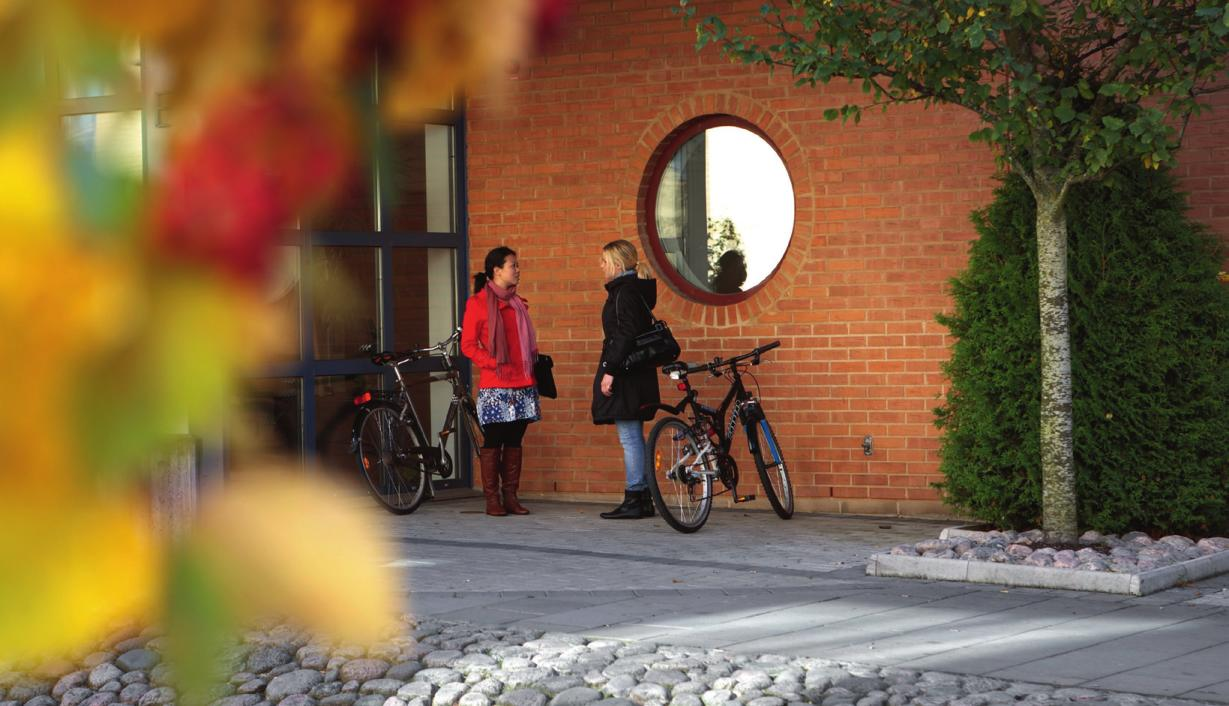
\includegraphics[width=\textwidth]{template/Manuscript/foto.jpg}
\caption{A figure with a long caption. Sed commodo posuere pede. Mauris ut est. Ut quis purus. Sed ac odio.
Sed vehicula hendrerit sem. Duis non odio. Morbi ut dui. Sed accumsan risus eget odio.
In hac habitasse platea dictumst. Pellentesque non elit. Fusce sed justo eu urna porta tincidunt.
Mauris felis odio, sollicitudin sed, volutpat a, ornare ac, erat.}
\label{fig:first_figure}
\end{figure}

Here are examples of a bullet list using the itemize environment:

\begin{itemize}
    \item First item with itemize
    \item Second item
    \item Third item
\end{itemize}

And heres an enumerate environment:

\begin{enumerate}
    \item First item with enumerate
    \item Second item
    \item Third item
\end{enumerate}

If you need footnotes, use the \verb|\footnote{}| command and they will appear looking like this\footnote{This is a footnote.}.

\lipsum[6-8]

\section{Outline}
\label{sec:outline}

\lipsum[11]